\section{User Application}

\subsection{Functional Requirements}

	\begin{flushleft}
		\begin{itemize}
			\item{\textbf{R5:}} FMDS will provide an interface for the ranger to initialise the drone.
				\begin{itemize}
					\item Discussed in previous functional requirement (R1.1.2).
				\end{itemize} 
			\item{\textbf{R6:}} FMDS will provide an interface to display snapshots of the video feed.
				\begin{itemize}
					\item The periodic snapshots (which will be used to generate the virtual 2D map) will be accessible via the application.
				\end{itemize} 
			\item{\textbf{R7:}} FMDS will provide an interface to display the live video feed.
				\begin{itemize}
					\item The live video feed coming from the drone will be accessible via the application.
				\end{itemize} 
			\item{\textbf{R8:}} FMDS will retrieve map and pin data from the server.
				\begin{itemize}
					\item Discussed in previous functional requirement (R2.2.1).
				\end{itemize} 
			\item{\textbf{R9:}} FMDS will provide an interface for the ranger to select a predefined flight pattern.
				\begin{itemize}
					\item Discussed in previous functional requirement (R2.1).
				\end{itemize} 
			\item{\textbf{R10:}} FMDS will provide a user interface for the notification received from the other subsystems.
				\begin{itemize}
					\item The notification received will include the relative position to the detected object from the drone's location.
				\end{itemize} 
		\end{itemize}

	\end{flushleft}

\subsection{Use Case Diagram}
	\begin{center}
		\begin{figure}[h!]
			\centering
			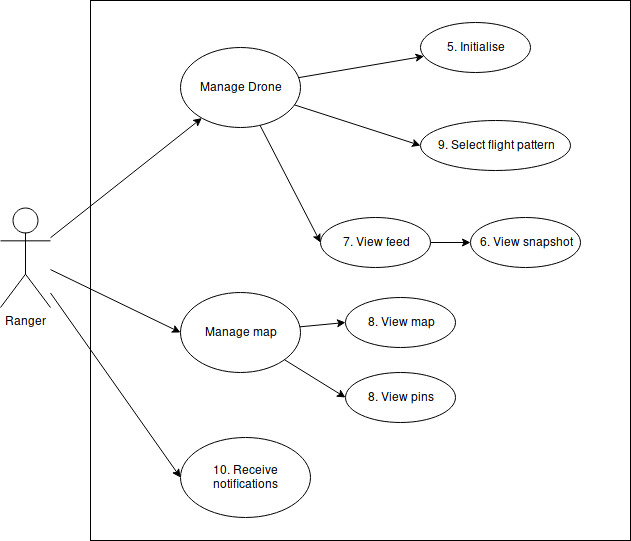
\includegraphics[scale=0.45]{./assets/images/application-ucd.jpg}
			\label{fig: user-application-ucd }
			\caption{User Application Use Case Diagram}
		\end{figure}
	\end{center}

\subsection{Technical Requirements}
	\begin{flushleft}
		\begin{itemize}
				\item Ionic cross platform framework.
				\item Cordova compilation suite.
				\item Angular Framework.
		\end{itemize}
	\end{flushleft}
